\documentclass{minimal}

\usepackage{tikz}
\usetikzlibrary{
	arrows.meta,
	decorations.pathmorphing,
	backgrounds,
	positioning,
	fit,
	petri,
	shapes.misc,
	graphs,
	quotes,
	decorations.pathreplacing,
	calc,
}

%\input{tikz_styles.tex}  % styles used in figures
\tikzset{infectious/.style={
		% The shape:
		rectangle,rounded corners=2mm,
		% The size:
		minimum size=8mm,
		% The border:
		very thick,
		draw=red!50!black!50, % 50% red and 50% black,
		% and that mixed with 50% white
		% The filling:
		top color=white, % a shading that is white at the top...
		bottom color=red!50!black!20, % and something else at the bottom
		% make sure text aligns properly 
		text height=1.5ex,text depth=.25ex,
}}

\tikzset{noninfectious/.style={
		% The shape:
		rectangle,rounded corners=2mm,
		% The size:
		minimum size=8mm,
		% The rest
		very thick,draw=black!50,
		top color=white,bottom color=black!20,
		% make sure text aligns properly 
		text height=1.5ex,text depth=.25ex,
}}

\tikzset{supinfectious/.style={
		% The shape:
		rectangle,rounded corners=2mm,
		% The size:
		minimum size=9.5mm,
		% The border:
		very thick,
		draw=red!50!black!50, % 50% red and 50% black,
		% and that mixed with 50% white
		% The filling:
		top color=white, % a shading that is white at the top...
		bottom color=red!50!black!20, % and something else at the bottom
		% make sure text aligns properly 
		text height=1.5ex,text depth=.25ex,
}}

\tikzset{supnoninfectious/.style={
		% The shape:
		rectangle,rounded corners=2mm,
		% The size:
		minimum size=9.5mm,
		% The rest
		very thick,draw=black!50,
		top color=white,bottom color=black!20,
		% make sure text aligns properly 
		text height=1.5ex,text depth=.25ex,
}}

\begin{document}
	
	\pagestyle{empty}
	
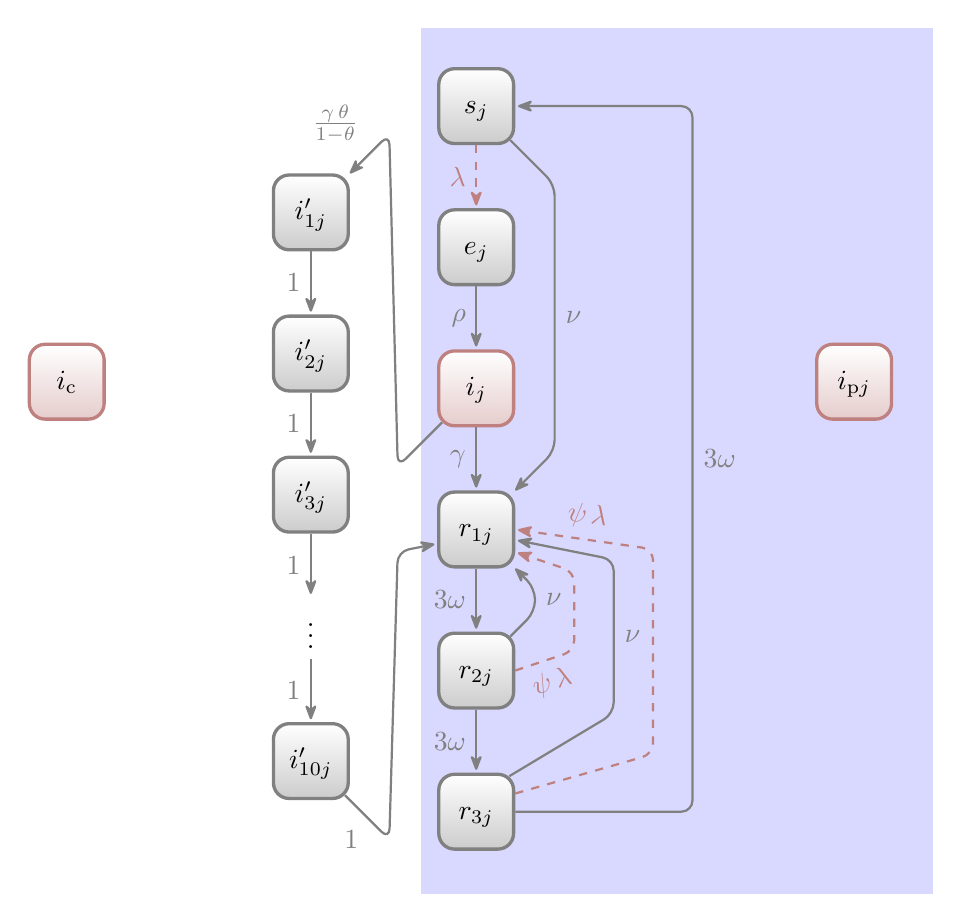
\begin{tikzpicture}[>={Stealth[round]},thick,black!50,text=black,
	every new ->/.style={shorten >=1pt},
	graphs/every graph/.style={edges=rounded corners}]
	\graph [grow down sep=8mm, branch right=7mm] {
		ic/"$i_{\mathrm{c}}$" [supinfectious,yshift=-35mm] {"$i_{\mathrm{c}}$"};
		ipr1/"$i^{\prime}_{1j}$" [supnoninfectious,xshift=24mm,yshift=-13.5mm] {"$i^{\prime}_{1j}$"} ->[black!50,"$1$"'] 
		ipr2/"$i^{\prime}_{2j}$" [supnoninfectious,xshift=24mm,yshift=-13.5mm] {"$i^{\prime}_{2j}$"} ->[black!50,"$1$"'] 
		ipr3/"$i^{\prime}_{3j}$" [supnoninfectious,xshift=24mm,yshift=-13.5mm] {"$i^{\prime}_{3j}$"} ->[black!50,"$1$"'] 		
		ipvdots/"$\vdots$" [xshift=24mm,yshift=-13.5mm] {"$\vdots$"} ->[black!50,"$1$"'] 
		ipr10/"$i^{\prime}_{10j}$" [supnoninfectious,xshift=24mm,yshift=-13.5mm] {"$i^{\prime}_{10j}$"};
		s/"$s_j$" [supnoninfectious,xshift=38mm] {"$s_j$"}->[dashed,red!50!black!50,"$\lambda$"']
		e/"$e_j$" [supnoninfectious,xshift=38mm] {"$e_j$"} ->[black!50,"$\rho$"']
		i/"$i_j$" [supinfectious,xshift=38mm] {"$i_j$"} ->[black!50,"$\gamma$"']		
		r1/"$r_{1j}$" [supnoninfectious,xshift=38mm] {"$r_{1j}$"} ->[black!50,"$3\omega$"']
		r2/"$r_{2j}$" [supnoninfectious,xshift=38mm] {"$r_{2j}$"} ->[black!50,"$3\omega$"']
		r3/"$r_{3j}$" [supnoninfectious,xshift=38mm] {"$r_{3j}$"};
		ip/"$i_{\mathrm{p}j}$" [supinfectious,xshift=79mm,yshift=-35mm] {"$i_{\mathrm{p}j}$"};
	};
	[font=\sffamily\bfseries,align=center,text width=3cm] {Healthcare workers};
	\draw [->,rounded corners,shorten <= -2.5pt] ($(s.south east)$) -- ($ (s.south east) + (5mm,-5mm) $) to [edge label=$\nu$,color=black!50] ($ (r1.north east) + (5mm,5mm) $) -- ($ (r1.north east) $);
	\draw [->,rounded corners,shorten <= -2.5pt] ($(i.south west)$) -- ($ (i.south west) + (-5mm,-5mm) $) -- ($ (ipr1.north east) + (5mm,5mm) $) to [edge label'=$\frac{\gamma\,\theta}{1-\theta}$,color=black!50] ($ (ipr1.north east) $);
	\draw [->,rounded corners,shorten <= -2.5pt,shorten >= 1pt] ($(ipr10.south east)$) to [edge label'=$1$,color=black!50] ($ (ipr10.south east) + (5mm,-5mm) $) -- ($ (r1.200) + (-5mm,-1mm) $) -- ($ (r1.200) $);
	\draw [->,rounded corners,shorten <= -2.5pt] ($(r2.north east)$) -- ($ (r2.north east) + (2.5mm,2.5mm) $) to [edge label'=$\nu$,color=black!50] ($ (r1.south east) + (2.5mm,-2.5mm) $) -- ($ (r1.south east) $);
	\draw [->,rounded corners,shorten >= 1pt,dashed,red!50!black!50,] ($(r2.east)$) to [edge node={node [sloped,below] {$\psi\,\lambda$}}] ($ (r2.east) + (7.5mm,2.5mm) $) -- ($ (r1.330) + (7.5mm,-2.5mm) $) -- ($ (r1.330) $);
	\draw [->,rounded corners,shorten <= -2.5pt,shorten >= 1pt] ($(r3.north east)$) -- ($ (r3.north east) + (12.5mm,7.5mm) $) to [edge label'=$\nu$,color=black!50] ($ (r1.345) + (12.5mm,-2.5mm) $) -- ($ (r1.345) $);
	\draw [->,rounded corners,shorten >= 1pt,dashed,red!50!black!50,] ($(r3.25)$) -- ($ (r3.25) + (17.5mm,5mm) $) -- ($ (r1.east) + (17.5mm,-2.5mm) $) to [edge node={node [sloped,above] {$\psi\,\lambda$}}] ($ (r1.east) $);
	\draw [->,rounded corners,shorten >= 1pt] ($(r3.east)$) -- ($ (r3.east) + (22.5mm,0mm) $) to [edge label'=$3\omega$,color=black!50] ($ (s.east) + (22.5mm,0mm) $) -- ($ (s.east) $);
	\begin{scope}[on background layer={color=blue!15}]
		\fill (4.5,0.5) rectangle (11,-10.5);
	\end{scope}
\end{tikzpicture}

	
\end{document}



